\documentclass[11pt]{article}
\usepackage[utf8]{inputenc}
\usepackage{minimalist}
\usepackage{graphicx}
\usepackage{multicol}
\usepackage{array}

\title{\textbf{Matrice (2D nizovi)}\\[4pt]\large Predavanje 10}
\date{}

\renewcommand{\figurename}{Slika}

\begin{document}
\maketitle
\thispagestyle{fancy}
\markboth{Matrice — Predavanje 10}{}

% ═════════════════════════════════════════════════════════════════════════
\section*{Zagrijavanje: Leksikografski redoslijed}

Možemo li uporediti dvije riječi znakovima $>$ i $<$? Možemo li reći da je \texttt{"drvored" < "drvosjeca"}? 
Na prvu možda nema smisla, ali odgovor je da! Ako imamo dvije riječi $X$ i $Y$, veća je ona koja dolazi kasnije u 
rječniku. To zovemo leksikografskim poređenjem.

Kako bismo utvrdili koja riječ dolazi prije u rječniku, vršimo poređenje slovo po slovo, s lijeva na desno:

\begin{enumerate}
    \item Nađemo prvu poziciju na kojoj se slova razlikuju.
          Koja god riječ ima \emph{abecedno manje} slovo na toj poziciji — ta dolazi prva.
    \item Ako smo došli do kraja jedne od riječi a nismo pronašli razliku — \emph{kraća} dolazi prva.
    \item Ako ne postoji razlika niti među slovima niti u dužini riječi, one su jednake.
\end{enumerate}

\begin{center}
\begin{tabular}{@{} >{\ttfamily}l l l @{}}
    \toprule
    \textbf{Poređenje} & \textbf{Razlika} & \textbf{Rezultat} \\
    \midrule
    "suncokret" vs "zub" & pozicija 0: \texttt{s} < \texttt{z} & "suncokret" $<$ "zub" \\
    "ajvar" vs "avion"  & pozicija 1: \texttt{j} < \texttt{v} & "ajvar" $<$ "avion" \\
    "drvo"  vs "drvored" & "drvo" je prefiks, kraće & "drvo" $<$ "drvored" \\
    \bottomrule
\end{tabular}
\end{center}

\smallskip
U C++-u, stringovi se porede operatorima \texttt{<}, \texttt{>}, \texttt{==}
i automatski koriste leksikografski redoslijed:

\begin{lstlisting}
string a = "ajvar", b = "avion";
if (a < b) cout << a << " dolazi prije " << b;
\end{lstlisting}

Naš prvi zadatak bio je da iskucamo kod kojim vršimo ovo poređenje "ručno" - bez upotrebe 
operatora \texttt{<}, \texttt{>}, \texttt{==} nad stringovima.

Ispod je rješenje na koje smo nadošli.

\begin{lstlisting}
string prva_rijec, druga_rijec;
cout << "Upisati dvije rijeci razdvojene razmakom:" << endl;
cin >> prva_rijec >> druga_rijec;

int prvo_slovo_razlike = -1;

// Uporedjujemo slova, jedno po jedno, s lijeva na desno dok nam ne 
// ponestane slova u jednoj od rijeci
for (int i = 0; i < min(prva_rijec.length(), druga_rijec.length()); i++) {
    if (prva_rijec[i] == druga_rijec[i]) {
        continue;
    } else {
        prvo_slovo_razlike = i;
        break;
    }
}

// Nismo pronasli razliku izmedju rijeci, potrebno je provjeriti koja je kraca
if (prvo_slovo_razlike == -1) {
    if (prva_rijec.length() < druga_rijec.length()) {
        cout << prva_rijec << " dolazi prije " << druga_rijec << endl;
    } else if (prva_rijec.length() > druga_rijec.length()) {
        cout << prva_rijec << " dolazi poslije " << druga_rijec << endl;
    } else {
        cout << "Rijeci su iste" << endl;
    }
} 
// Pronasli smo razliku izmedju rijeci na indeksu prvo_slovo_razlike
else if (prva_rijec[prvo_slovo_razlike] < druga_rijec[prvo_slovo_razlike]) {
    cout << prva_rijec << " dolazi prije " << druga_rijec << endl;
} else if (prva_rijec[prvo_slovo_razlike] > druga_rijec[prvo_slovo_razlike]) {
    cout << prva_rijec << " dolazi poslije " << druga_rijec << endl;
}
\end{lstlisting}

\newpage

% ═════════════════════════════════════════════════════════════════════════
\section*{Matrice (2D nizovi, \textit{engl.} matrix)}

Matricu definišemo kao \textbf{vektor vektora}. Broj redova je \texttt{n},
broj kolona je \texttt{m}:

\begin{lstlisting}
// Matrica od n redova i m kolona, popunjena nulama
vector<vector<int>> matrica(n, vector<int>(m, 0));

// Matrica od n redova i m kolona, popunjena brojem 5
vector<vector<int>> matrica(n, vector<int>(m, 5));

// Matrica od n redova i m kolona, popunjena znakom '.'
vector<vector<char>> matrica(n, vector<int>(m, '.'));
\end{lstlisting}

\medskip
Čitanje matrice s ulaza radi se sa dvije ugniježdene petlje —
vanjska prolazi kroz \textbf{redove}, unutarnja kroz \textbf{kolone}:

\begin{lstlisting}
int n, m;
cin >> n >> m;

vector<vector<int>> matrica(n, vector<int>(m, 0));

for (int i = 0; i < n; i++) {
    for (int j = 0; j < m; j++) {
        cin >> matrica[i][j];
    }
}
\end{lstlisting}

\begin{napomena}
    Elementi na ulazu ne moraju biti u istom redu — \texttt{cin} automatski
    preskače razmake i nove redove. Dakle, ulaz možemo pisati red po red ili
    sve u jednom redu.
    Npr. u gornjem kodu, naredni ulazi predstavljaju istu matricu: \\
    \texttt{2 3}\\
    \texttt{1 2 3}\\
    \texttt{4 5 6}\\
    i \\
    \texttt{2 3}\\
    \texttt{1 2 3 4 5 6}
\end{napomena}


\newpage

% ═════════════════════════════════════════════════════════════════════════
\section*{Zadaci}


\begin{zadatak}{1 — Razlika dijagonala}
Data je kvadratna matrica dimenzija $n \times n$.
Izračunaj apsolutnu razliku sume \emph{glavne dijagonale}
(elementi $i = j$) i sume \emph{sporedne dijagonale}
(elementi $i + j = n - 1$).

\medskip
\begin{minipage}[t]{0.45\textwidth}
\textbf{Ulaz}\\[2pt]
U prvom redu broj $n$.\\
U narednih $n$ redova, po $n$ cijelih brojeva.

\medskip
\textbf{Izlaz}\\[2pt]
Jedan cijeli broj — apsolutna razlika suma dviju dijagonala.
\end{minipage}
\hfill
\begin{minipage}[t]{0.48\textwidth}
\textbf{Primjer}\\[2pt]
\begin{tabular}{@{}ll@{}}
\textit{Ulaz} & \textit{Izlaz} \\
\begin{minipage}[t]{2.5cm}
\ttfamily\small
3\\
1 2 3\\
4 5 6\\
7 8 9
\end{minipage}
&
\begin{minipage}[t]{2cm}
\ttfamily\small
0
\end{minipage}
\end{tabular}

\medskip
Glavna: $1{+}5{+}9=15$, sporedna: $3{+}5{+}7=15$, razlika: $|15-15|=0$.
\end{minipage}
\end{zadatak}


\subsection*{Rješenje zadatka 1}

\begin{figure}[h]
    \centering
    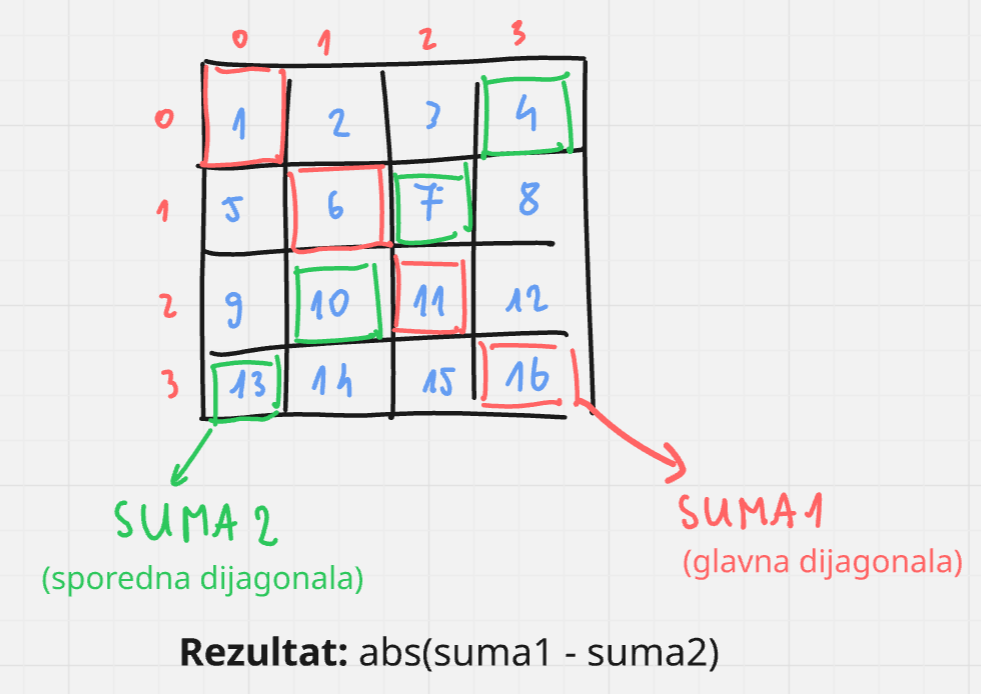
\includegraphics[width=0.5\linewidth]{rjesenje1.png}
    \caption{Objašnjenje zadataka. Glavna dijagonala je ona za koju vrijedi i = j (crvena). 
    Sporedna je ona za koju vrijedi i + j = n - 1 (zelena). Zadatak traži da izračunamo
    sumu brojeva na glavnoj dijagonali, sumu na sporednoj te ih oduzmemo i ispišemo apsolutnu
    vijednost razlike.}
    \label{fig:placeholder}
\end{figure}

Kod koji smo napisali na času izgledao je ovako:

\begin{lstlisting}
// Unos matrice
int n;
cout << "Unijeti velicinu kvadrata: " << endl;
cin >> n;
cout << "Unijeti kvadrat: " << endl;

vector<vector<int> >  kvadrat(n, vector<int>(n, -1));
for (int i = 0; i < n; i++) {
    for (int j = 0; j < n; j++) {
        cin >> kvadrat[i][j]; 
    }
}

// Sabiranje brojeva na dijagonalama
int suma_dijagonale1 = 0, suma_dijagonale2 = 0;
for (int i = 0; i < n; i++) {
    for (int j = 0; j < n; j++) {
        if (i == j) {
            suma_dijagonale1 += kvadrat[i][j];
        }
        
        if (i + j == n - 1) {
            suma_dijagonale2 += kvadrat[i][j];
        }
    }
}
cout << abs(suma_dijagonale1 - suma_dijagonale2) << endl;
\end{lstlisting}

Postoji još jedno, kraće, rješenje ovoga zadatka koje koristi činjenicu da ako znamo koorindatu $i$ nekog polja, onda
znamo i vrijednost koordinate $j$ ako mora biti na glavoj/sporednoj dijagonali. 

Ako je polje na glavnoj dijagonali onda će vrijednost $j$ biti jednaka $i$, a ako je na sporednoj onda će iz $i + j = n - 1$ vrijediti $j = n - 1 - i$.

\begin{lstlisting}
// Unos matrice
...

// Sabiranje brojeva na dijagonalama
for (int i = 0; i < n; i++) {
    suma_dijagonale1 += kvadrat[i][i];
    suma_dijagonale2 += kvadrat[i][n - 1 - i];
}
cout << abs(suma_dijagonale1 - suma_dijagonale2) << endl;
\end{lstlisting}

\newpage

% ═════════════════════════════════════════════════════════════════════════
\section*{Domaća zadaća}

\vspace{0.5cm}

\begin{zadatak}{1 — Magični kvadrat}
Data je kvadratna matrica dimenzija $n \times n$.
Ispiši sumu svakog reda, sumu svake kolone, te sumu
\emph{glavne dijagonale} (elementi za koje vrijedi $i = j$).

\medskip
\begin{minipage}[t]{0.45\textwidth}
\textbf{Ulaz}\\[2pt]
U prvom redu broj $n$.\\
U narednih $n$ redova, po $n$ cijelih brojeva.

\medskip
\textbf{Izlaz}\\[2pt]
$n$ redova za sume redova,\\
$n$ redova za sume kolona,\\
jedan red za sumu dijagonale.
\end{minipage}
\hfill
\begin{minipage}[t]{0.48\textwidth}
\textbf{Primjer}\\[2pt]
\begin{tabular}{@{}ll@{}}
\textit{Ulaz} & \textit{Izlaz} \\
\begin{minipage}[t]{3cm}
\ttfamily\small
3\\
2 7 6\\
9 5 1\\
4 3 8
\end{minipage}
&
\begin{minipage}[t]{4.5cm}
\ttfamily\small
Suma reda 0 je 15\\
Suma reda 1 je 15\\
Suma reda 2 je 15\\
Suma kolone 0 je 15\\
Suma kolone 1 je 15\\
Suma kolone 2 je 15\\
Suma dijagonale je 15
\end{minipage}
\end{tabular}
\end{minipage}
\end{zadatak}

\begin{zadatak}{2 — Ogledalo}
Data je matrica karaktera dimenzija $n \times m$.
Napravi novu matricu čiji će elementi biti isti kao elementi početne matrice, ali u kojoj je 
svaki red napisan naopako.
Ispiši novu matricu, a ispod nje, ispiši originalnu i novu matricu
jednu pored druge (spojene u isti red).

\medskip
\begin{minipage}[t]{0.45\textwidth}
\textbf{Ulaz}\\[2pt]
Red sa $n$ i $m$.\\
Narednih $n$ redova, po $m$ cijelih brojeva.

\medskip
\textbf{Izlaz}\\[2pt]
Zrcaljena matrica,\\
prazan red,\\
matrica \textquotedblleft spojena\textquotedblright\ (original~|~nova).
\end{minipage}
\hfill
\begin{minipage}[t]{0.48\textwidth}
\textbf{Primjer}\\[2pt]
\begin{tabular}{@{}ll@{}}
\textit{Ulaz} & \textit{Izlaz} \\
\begin{minipage}[t]{2.5cm}
\ttfamily\small
3 3\\
x * x\\
. x *\\
. . x
\end{minipage}
&
\begin{minipage}[t]{3.6cm}
\ttfamily\small
x * x

* x .

x . .\\

x * x x * x\\
. x * * x .\\
. . x x . .
\end{minipage}
\end{tabular}
\end{minipage}
\end{zadatak}

% ═════════════════════════════════════════════════════════════════════════

% \begin{mdframed}[linecolor=accent!40, linewidth=0.8pt, backgroundcolor=accent!3,
%                  innertopmargin=80pt, innerbottommargin=12pt]
%     \color{gray}\small\textit{[Domaća zadaća — dodati naknadno]}
% \end{mdframed}

\end{document}
